%\vspace{2mm}

\section{Experiments and results}

This section describes the dataset used to evaluate the proposed architecture, and the results of the different experiments carried out with it. All experiments were conducted on a desktop Intel i7-7700 CPU machine at 3.60GHz and a GeForce GTX 950 GPU, and implemented in Python. The thresholds of the system, $\lambda_{IOU}$ and $\lambda_{FBTR}$, were set based on a private collection of training videos to 0.25 and 0.7, respectively.

\subsection{Evaluation dataset}

\begin{table*}[h!]
    \centering
    \small
    \begin{tabular}{ccccccccc}
        \toprule
         & Resolution & Length & Face dets. & Density & Scenario & \#Subjects & Description \\
         \midrule
        Choke1 & 800x600 & 1'24" & 7964 & 4.0 & Indoor & 24 (*) & Corridor recorded from 3 cameras over a door.\\
        Choke2 & 800x600 & 1'11" & 8710 & 4.8 & Indoor & 26 (*) & Corridor recorded from 3 cameras over a door.\vspace{1mm}\\
        Street & 1920x1080 & 1'8" & 4883 & 2.9 & Outdoor & 31 & Street scene filmed from a low-eye level angle.\\
        Sidewalk & 1920x1080 & 27" & 8433 & 13.0 & Outdoor & 34 &  Crowd walking to the camera, filmed at eye level.\\
        Bengal & 1920x1080 & 40" & 6953 & 6.9 & Outdoor & 36 & A pedestrian scene filmed at eye level.\\
         \bottomrule
    \end{tabular}
    \caption{Description of the videos used to evaluate our tracking architecture. In videos marked with asterisk (*), subjects leave and re-enter the scene twice. Density refers to the mean number of face detections per frame.}
    \label{tab:videos}
\end{table*}

Since there are no public datasets fully corresponding to our use case (c.f. Section \ref{sec:public_datasets}), we have compiled and annotated a set of 5 videos showing  crowded indoor and outdoor video-surveillance scenes. 

Two of these videos come from the extra sequences (cameras P2E\_S5 and P2L\_S5) of the well-known public dataset ChokePoint \cite{wong2011chokepoint}. To force re-appearances of subjects and validate the FBTR module performance, the three sequences recorded by P2E\_S5 cameras were concatenated, leading to the \textit{Choke1} video. Similarly, the video \textit{Choke2} was generated from \textit{P2L\_S5} cameras sequences. The remaining three videos were selected from YouTube. Table \ref{tab:videos} details each video content and properties.

Tracks were semi-automatically annotated to obtain ground truth data. Firstly, face bounding boxes were retrieved using a state-of-the-art face detector \cite{zhang2017faceboxes}. Only faces with a detection confidence above 0.50 were considered. Then, detections were manually verified, and tracks and corresponding IDs were annotated\footnote{All videos and annotations are publicly available at \url{https://github.com/hertasecurity/LTFT}.}.


\subsection{Benchmarking of face trackers} 
\label{sec:STFT_benchmark}

This first experiment aims at benchmarking different trackers to choose the most appropriate one for the tracking module. We analyze the performance of our data association module using the following visual trackers: CSRT~\cite{lukezic2017discriminative}, KCF~\cite{bochinski2018viou}, Median Flow~\cite{kalal2010forward} and MOSSE~\cite{bolme2010visual}. Additionally, we include in our benchmark the longer-term tracker TLD \cite{kalal2010face} and the state-of-the-art deep tracker SiamRPN++~\cite{li2019siamrpn++}. 

Table~\ref{tab:results_STFT} and Figure~\ref{fig:stft_CRP} present the results obtained on all of our evaluation videos. Results highlight the lower performance of TLD. This is probably due to its capability to re-identify targets, which makes it vulnerable to ID-switches. The best performing tracker in terms of ID-switches is MOSSE, but its high fragmentation leads to a poor overall completion rate. The SiamRPN++ tracker achieves the highest completion rate ($CRS=0.590$) and the lowest fragmentation ($Frag=0.01264$). However, KCF is very close to it ($CRS=0.587$, $Frag=0.01299$) and runs at much higher FPS, which is critical in video-surveillance contexts. 

According to these findings, simple visual trackers and more sophisticated DL-based trackers lead to similar performances in such challenging environments where occlusions are extremely frequent. In the following experiments we will use the KCF tracker as the core of our tracking module.

\begin{table}[h]
    \centering
    \small
    \begin{tabular}{ccccc}
        \toprule
        Tracker & Frag & ID-Switches & CRS & FPS\\
        \midrule
        CSRT & 0.01326 & 0.00379 & 0.581 & 3.80\\
        KCF & 0.01299 & 0.00395 & \textbf{0.587} & \textbf{22.12}\\
        Median Flow & 0.01470 & 0.00352 & 0.574 & 16.26\\
        MOSSE & 0.21831 & \textbf{0.00192} & 0.234 & 21.63\\
        SiamRPN++ & \textbf{0.01264} & 0.00420 & \textbf{0.590} & 1.74\\
        TLD & 0.03711 & 0.00912 & 0.515 & 1.51\\
        \bottomrule
    \end{tabular}
    \caption{Evaluation of the data association module on the whole dataset, using different trackers in the tracking module.}
    \label{tab:results_STFT}
\end{table}

\begin{figure}[h]
    \centering
    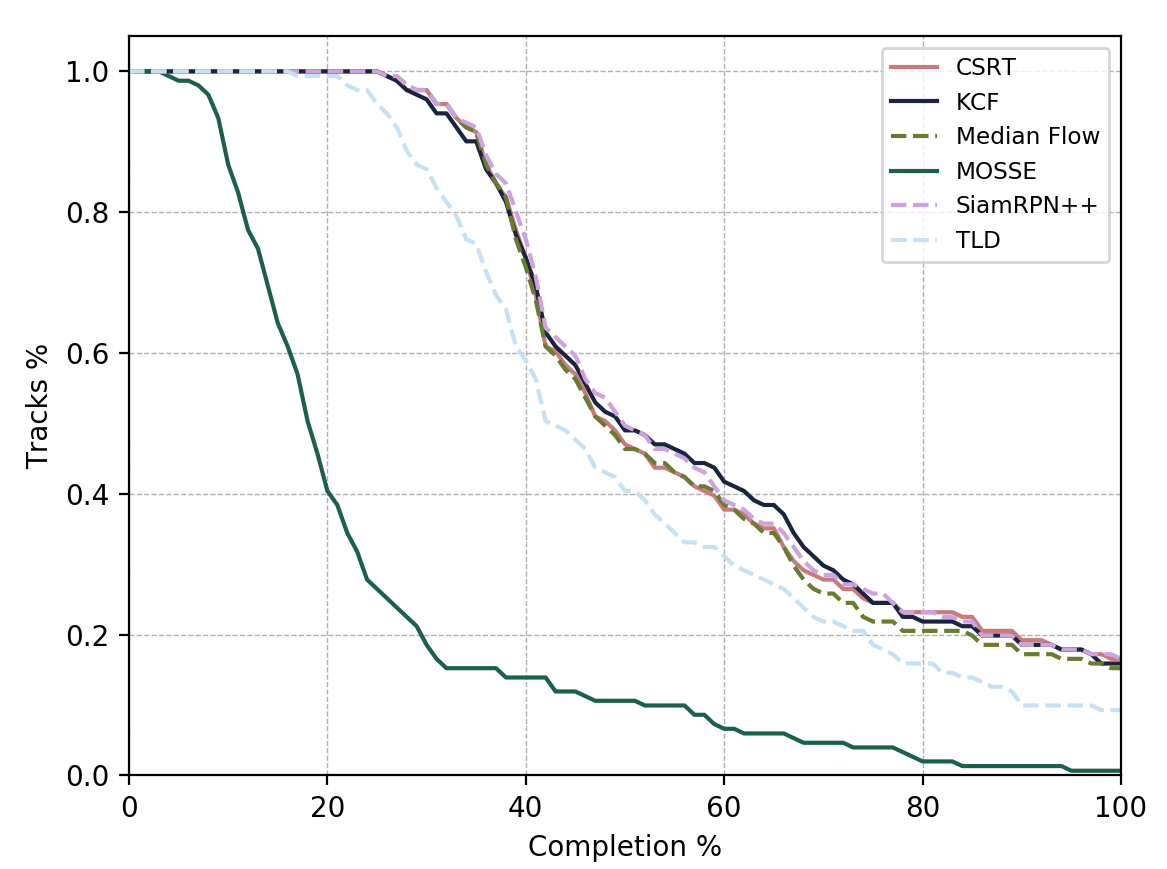
\includegraphics[width=\linewidth]{all_only_stft_completion_results}
    \caption{CRP for each tracker tested in the tracking module.}
    \label{fig:stft_CRP}
\end{figure}


\subsection{Ablation study}

In this section, we present an ablation study that quantifies the contribution of each module (TM, DA, FBTR and CM) and demonstrates the suitability of the proposed approach for long-term tracking in crowded video-surveillance scenarios.

Five ablation experiments are presented: 

\begin{itemize}
    \item \textbf{DA.} Tracking is performed following a simple data association strategy: the tracking module is deactivated, and data association is computed based on the IOU value of detections in consecutive frames.
    \item \textbf{DA+FBTR.} Same as DA, plus face identification.
    \item \textbf{DA+TM.} In this experiment, data association is carried out using KFC in the tracking module. No face identification or correction mechanisms are applied.
    \item \textbf{DA+TM+FBTR.} Same as DA+TM, plus FBTR.
    \item \textbf{DA+TM+FBTR+CM.} Same as DA+TM+FBTR, plus correction capabilities.
\end{itemize}


Table \ref{tab:ablation_ALL_table} and Figure \ref{fig:ablation_CRP} show the results of the ablation study on our whole dataset. It can be clearly observed that each added module increases the overall tracking completion rate. The impact of FBTR is particularly noteworthy: it increases the CRS by a 15.5\% (from 0.503 to 0.581) and a 12.2\% (from 0.587 to 0.659) when added to DA and DA+TM, respectively.
The correction module also improves long-term tracking (CRS increase of 11.5\%, from 0.659 to 0.735) without any extra computational cost. At the same time, it strongly reduces the fragmentation generated by the FBTR module by a 22.8\% (from 0.1573 to 0.1215). As expected, the number of ID-Switches increases as we achieve longer-term tracking, but its value stays reasonably low (0.00357 when FBTR is used).

Table \ref{tab:ablation_tables} details ablation results per video. 
Results on \textit{Choke1} and \textit{Choke2} highlight the good performance of our architecture, especially of the FBTR module (CRS increases above 50\%), in contexts where people leave and re-enter the scene. The impact of the CM is also dramatic, reaching CRS values up to 0.845 and reducing fragmentation up to 40\%.
The remaining videos do not contain subject re-appearances. In the case of  \textit{Sidewalk}, where long occlusions are frequent, FBTR and CM improve short-term tracking by a 7.3\% (CRS=0.718) and  11.2\% (CRS=0.744), respectively.
\textit{Street} and \textit{Bengal} are the most challenging videos in terms of illumination, motion and occlusions. In these videos, the impact of FBTR and CM is lower, but the DA+TM+FBTR+CM architecture is still the most successful one.


\begin{table}[t]
    \centering
    \small
    \begin{tabular}{lcccc}
        \toprule
        Tracking architecture & Frag & ID-Switches & CRS & FPS\\
        \midrule
        DA & 0.02677 & \textbf{0.00097} & 0.503 & \textbf{30.0}\\
        DA+FBTR & 0.02940 & 0.00114 & 0.581 & 12.9\\
        DA+TM & 0.01299 & 0.00395 & 0.587 & 22.1\\
        DA+TM+FBTR & 0.01573 & 0.00357 & 0.659 & 10.9\\
        DA+TM+FBTR+CM & \textbf{0.01215} & 0.00357 & \textbf{0.735} & 10.9\\
        \bottomrule
    \end{tabular}
    \caption{Results of the ablation study on our whole dataset.}
    \label{tab:ablation_ALL_table}
\end{table}

\begin{figure}[t]
    \centering
    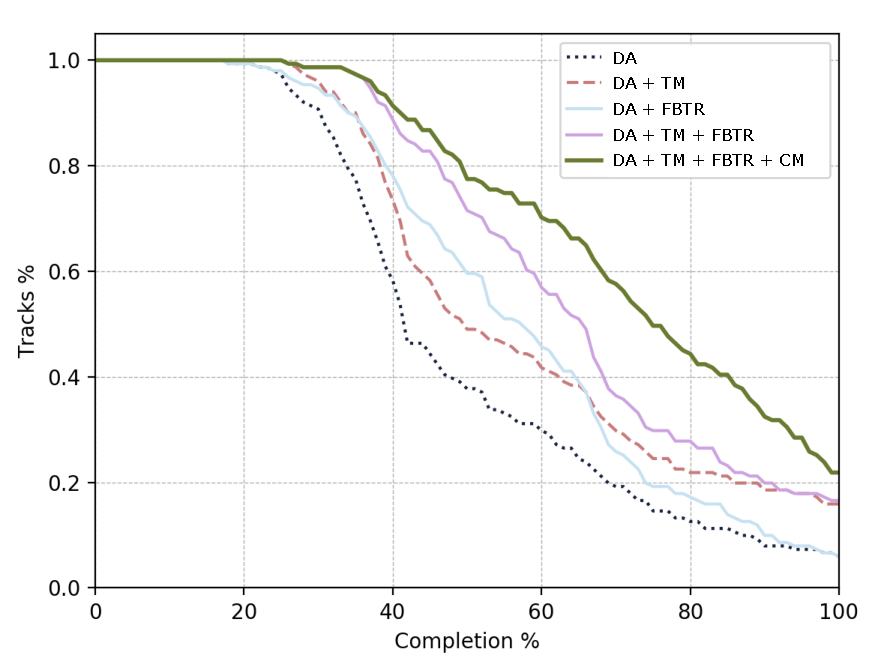
\includegraphics[width=\linewidth]{images/all_ablation_completion_results.pdf}
    \caption{CRPs for the different ablation experiments.}
    \label{fig:ablation_CRP}
\end{figure}

\begin{table}[t]
    \centering
    \small
    \begin{tabular}{lccccc}
        \toprule
        Choke1 (800x600) & Frag & ID-Switches & CRS & FPS\\
        \midrule
        DA & 0.01607 & \textbf{0.00001} & 0.375 & \textbf{50.4}\\
        DA+FBTR & 0.02022 & \textbf{0.00001} & 0.572 & 20.1\\
        DA+TM & 0.01017 & 0.00013 & 0.397 & 39.0\\
        DA+TM+FBTR & 0.01406 & 0.00013 & 0.605 & 17.1\\
        DA+TM+FBTR+CM & \textbf{0.00829} & 0.00013 & \textbf{0.720} & 17.1\\
        \midrule
        
        Choke2 (800x600) & & & &\\
        \midrule
        DA & 0.03387 & \textbf{0.00069} & 0.355 & \textbf{53.3}\\
        DA+FBTR & 0.03869 & 0.00103 & 0.511 & 18.1\\
        DA+TM & 0.01584 & 0.00253 & 0.400 & 34.3\\
        DA+TM+FBTR & 0.02124 & 0.00241 & 0.558 & 14.8\\
        DA+TM+FBTR+CM & \textbf{0.01447} & 0.00253 & \textbf{0.845} & 14.8\\
        \midrule
        
        Sidewalk (1920x1080) & & & &\\
        \midrule
        DA & 0.02929 & \textbf{0.00237} & 0.547 & \textbf{15.2}\\
        DA+FBTR & 0.03154 & 0.00261 & 0.618 & 4.7\\
        DA+TM & 0.00996 & 0.00984 & 0.669 & 9.2\\
        DA+TM+FBTR & 0.01150 & 0.00901 & 0.718 & 3.9\\
        DA+TM+FBTR+CM & \textbf{0.00949} & 0.00889 & \textbf{0.744} & 3.9\\
        \midrule
        
        Street (1920x1080) & & & &\\
        \midrule
        DA & 0.03031 & \textbf{0.00123} & 0.580 & \textbf{14.9}\\
        DA+FBTR & 0.03051 & 0.00143 & 0.577 & 13.8\\
        DA+TM & \textbf{0.01884} & 0.00410 & 0.634 & 15.6\\
        DA+TM+FBTR & 0.01946 & 0.00348 & 0.633 & 12.2\\
        DA+TM+FBTR+CM & \textbf{0.01925} & 0.00348 & \textbf{0.637} & 12.2\\
        \midrule
        
        Bengal (1920x1080) & & & &\\
        \midrule
        DA & 0.02459 & \textbf{0.00058} & 0.587 & \textbf{16.2}\\
        DA+FBTR & 0.02488 & \textbf{0.00058} & 0.607 & 7.8\\
        DA+TM & 0.01222 & 0.00288 & 0.732 & 12.5\\
        DA+TM+FBTR & 0.01323 & 0.00244 & 0.735 & 6.6\\
        DA+TM+FBTR+CM & \textbf{0.01194} & 0.00244 & \textbf{0.741} & 6.6\\
        \bottomrule
    \end{tabular}
    \caption{Results of ablation experiments per video.}
    \label{tab:ablation_tables}
\end{table}
